%MARCOS RIAL DOCAMPO
%Presentación en diapositivas del TFG

\documentclass[12pt]{beamer}
\usetheme{Madrid}
\usecolortheme{dolphin}
\useoutertheme{smoothbars}
\useinnertheme{circles}
\setbeamercovered{invisible}
\setbeamertemplate{navigation symbols}{}

\usepackage[utf8]{inputenc}
\usepackage[spanish]{babel}
\usepackage{helvet}
\usepackage{amsmath}
\usepackage{amsfonts}
\usepackage{amssymb}
\usepackage{latexsym}
\usepackage{graphicx}
\usepackage{hyperref}
\usepackage{url}
\usepackage{epstopdf}
%\usepackage{natbib}

\author[Marcos Rial Docampo]{Marcos Rial Docampo\\
	\footnotesize{Tutores:\\Eduardo Corbelle Rico y Rafael Enrique Corrales Andino}}
\title[Análisis de Separabilidad Espectral]{\large{Análisis de separabilidad espectral de especies\\de mangle en el Golfo de Fonseca}}
\subtitle{Aplicación a la clasificación de imágenes Landsat}

\institute[USC-EPS]{Trabajo Fin de Grado \\Universidad de Santiago de Compostela\\Escuela Politécnica Superior de Lugo} 
%\date{\today}
%\subject{}


% Directamente na páxina de título: \includegraphics antes de \maketitle
% \logo{\includegraphics[keyvals]{imagefile}}

%\AtBeginSection{
%\begin{frame}
 % \frametitle{Índice}
 % \tableofcontents[currentsection]
%\end{frame}
%}

%\AtBeginSubsection{ 
%\begin{frame}
%  \frametitle{Índice}
%  \tableofcontents[currentsection,currentsubsection]
%\end{frame}
%}

\begin{document}

\begin{frame}
\maketitle
\end{frame}

\section{Introducción}
\subsection{Marco Global}
\begin{frame}
\only<1>{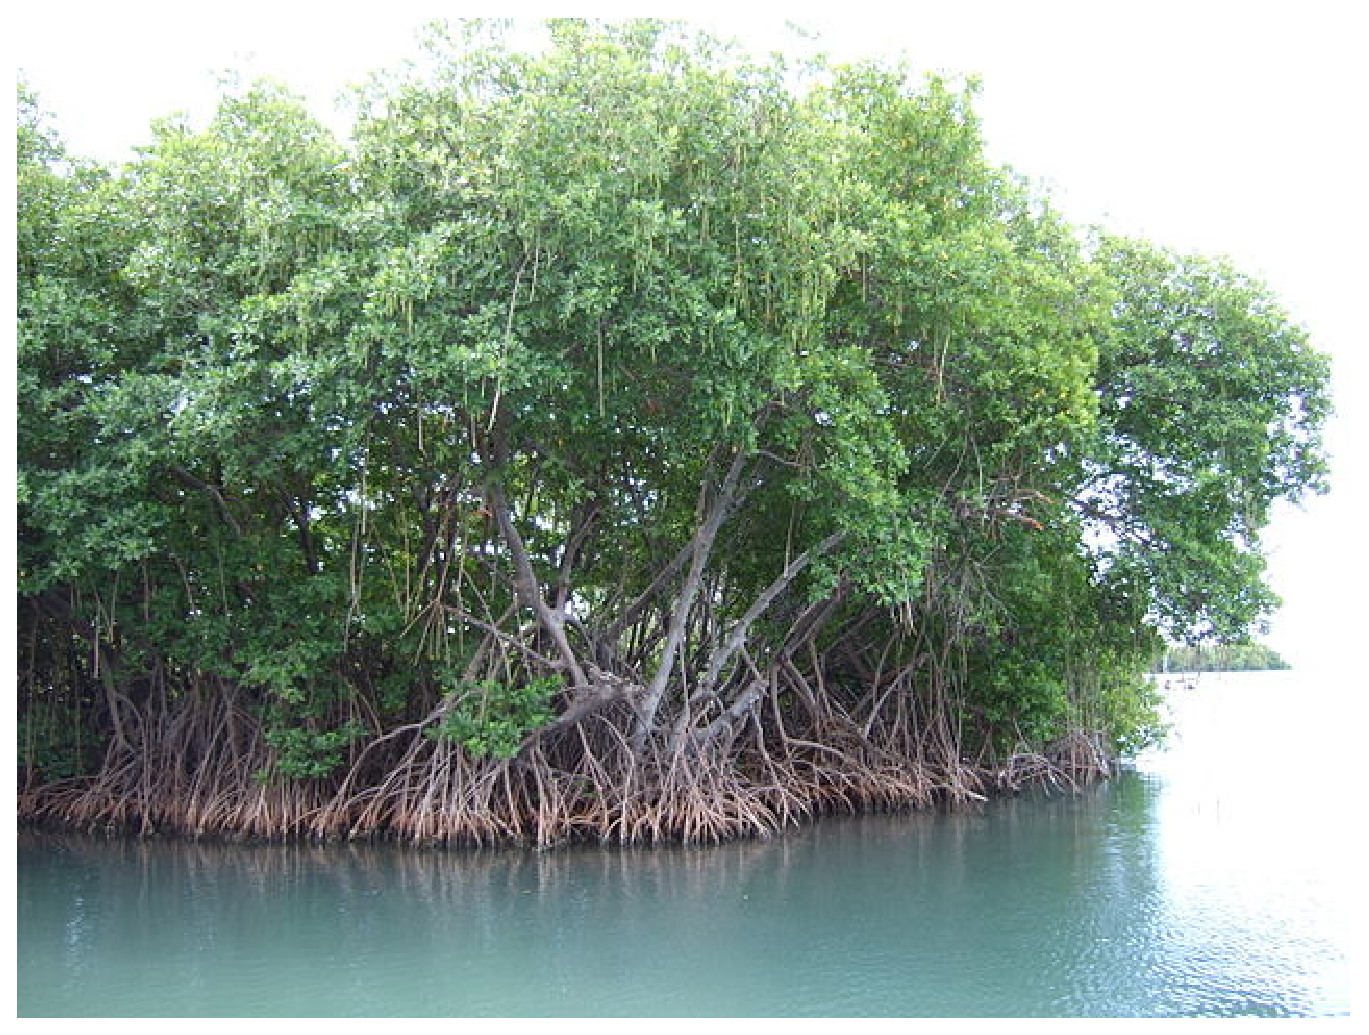
\includegraphics[width=\linewidth]{./Imagenes/Mangle.eps}}
\only<2>{\begin{block}{}
		\textbf{Manglar}: Ecosistema medioambiental propio de zonas costeras tropicales\\
		\textbf{Mangle}: Especie forestal que crece en los manglares o bosques de mangle
	\end{block}}
\end{frame}

\begin{frame}
\begin{block}{}
	\begin{itemize}
		\item Sistema medioambiental extenso y complejo \pause
		\item Situado en zona intermareal de zonas tropicales y subtropicales \pause
		\item Compuesto por más de 80 especies forestales y 2000 animales \pause
		\item Dependiente de procesos externos \pause
		\item Ecosistema gravemente amenazado
	\end{itemize}
\end{block}
\end{frame}

\subsection{Objetivos}
\begin{frame}
\begin{block}{Objetivos generales}
	\begin{enumerate}[<+->]
		\item Evaluar la posibilidad de emplear imágenes multiespectrales de satélite para diferenciar distintas especies de mangle del Golfo de Fonseca.
		\item La respuesta espectral de las diferentes especies es lo suficientemente diferente como para permitir la clasificación de estas imágenes.
	\end{enumerate}
\end{block}
\end{frame}

\begin{frame}
	\begin{block}{Objetivos específicos}
		\begin{enumerate}
			\item<1-> Análisis de separabilidad espectral de las especies:
				\begin{itemize}
					\item \textit{Rhizophora mangle} o mangle rojo
					\item \textit{Laguncularia racemosa} o mangle blanco
					\item \textit{Avicennia germinans} o mangle prieto
				\end{itemize}
			\item<2-> Realizar una clasificación de imágenes de Landsat 8\\
			\item<3-> Estudiar el empleo de software libre
		\end{enumerate}
	\end{block}
\end{frame}

\subsection{Zona de estudio}
\begin{frame}
\only<1>{\includegraphics[width=\linewidth]{./Imagenes/localizacion.eps}}
\only<2>{\includegraphics[width=\linewidth]{./Imagenes/localizacion_elev.eps}}
\end{frame}

\section{Material y Métodos}
\subsection{Estudio Radiométrico}
\begin{frame}
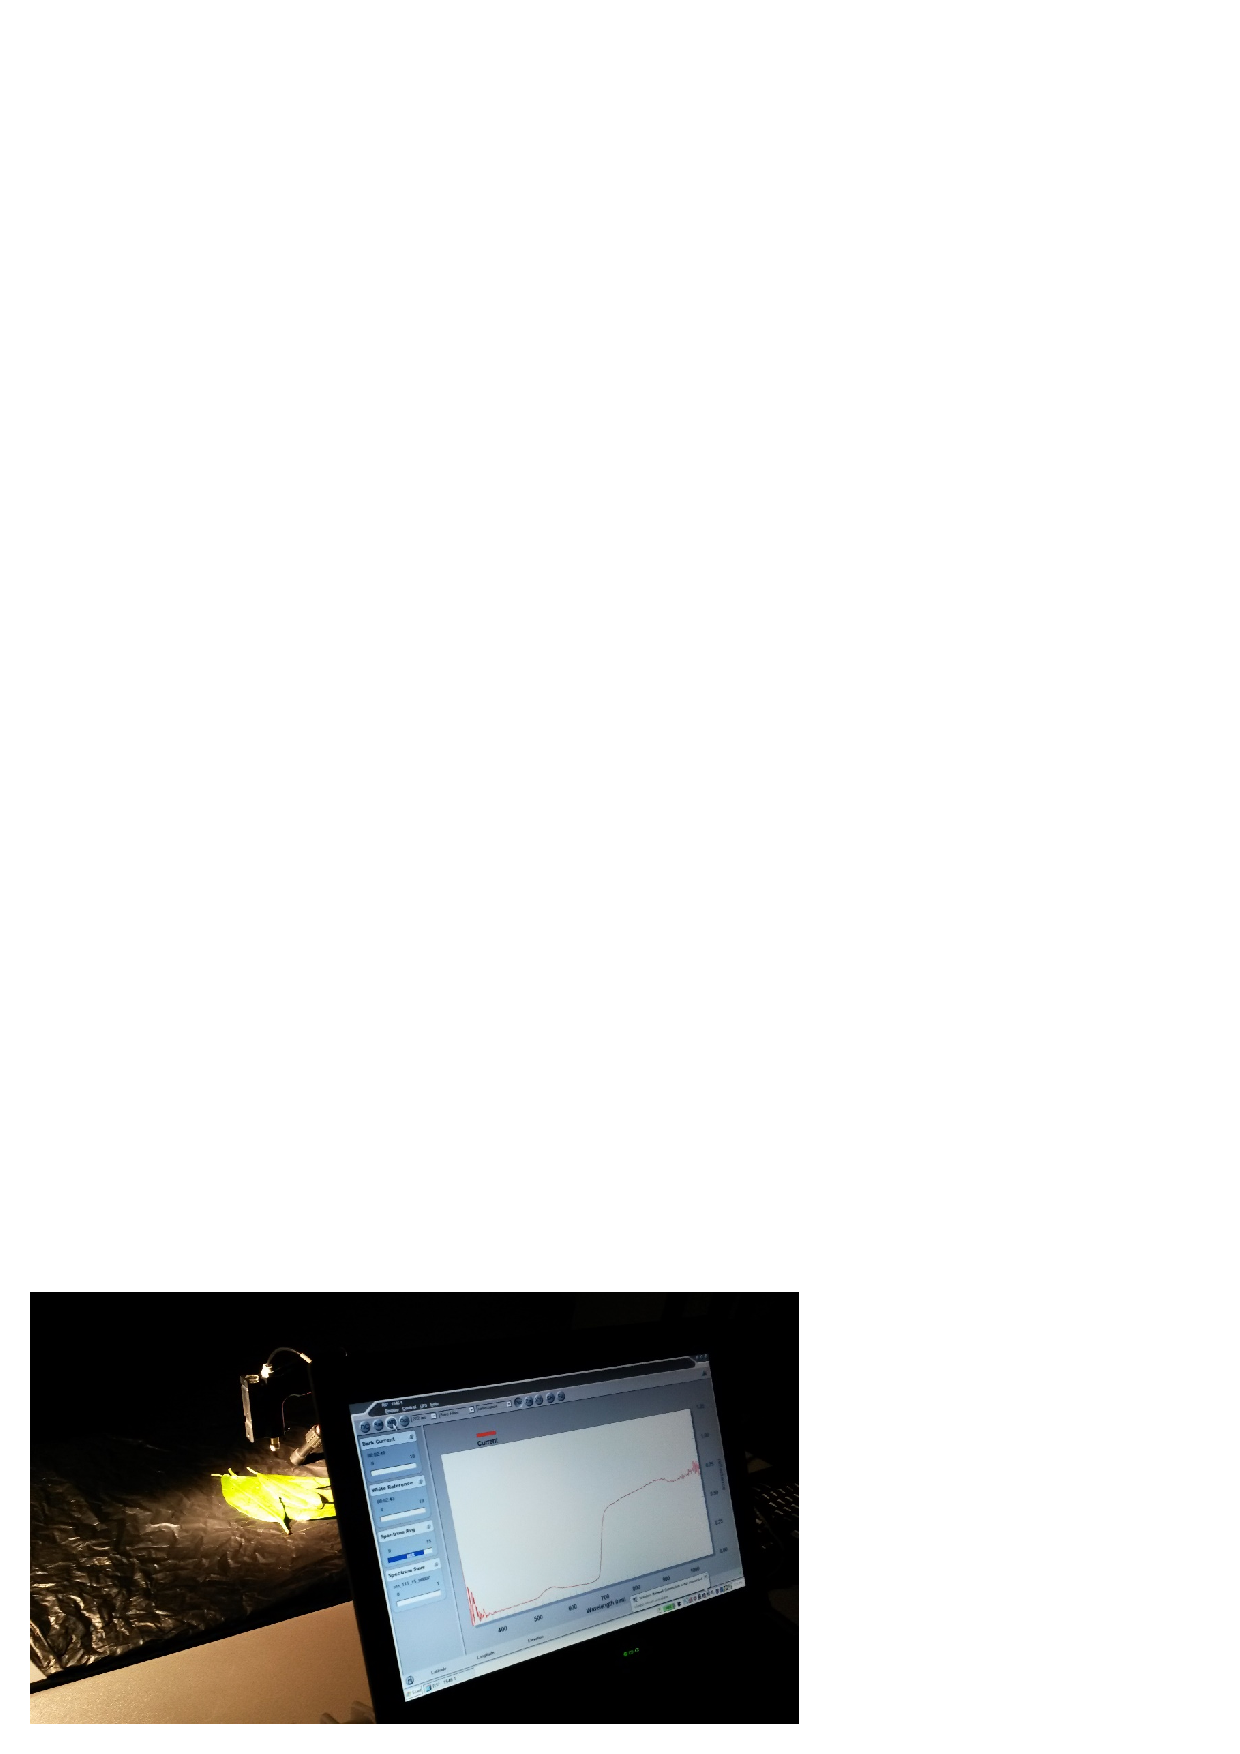
\includegraphics[width=\linewidth]{./Imagenes/Curva_espectral.jpg}
\end{frame}

\subsection{Software}
\begin{frame}
	\begin{columns}
		\begin{column}{3.5cm} \vspace*{0.2cm}
			\begin{block}{}
				\begin{itemize}[<+->]
					\item R
					\item GRASS GIS QGIS
					\item \LaTeX
					\item JabRef, SmartGit
				\end{itemize}
			\end{block}
		\end{column}
		\begin{column}{7cm}
			\begin{block}{}
			\only<4> {\small	\url{https://github.com/MarcosRial/TFG}}
			\end{block}
		\end{column}
	\end{columns}
	
\end{frame}

\section{Resultados}
\subsection{Análisis de Separabilidad}
\begin{frame}
	\only<1>{\includegraphics[width=\linewidth]{./Graficos/1.png}}
	\only<2>{\includegraphics[width=\linewidth]{./Graficos/2.png}}
	\only<3>{\includegraphics[width=\linewidth]{./Graficos/3.png}}
	\only<4>{\includegraphics[width=\linewidth]{./Graficos/4.png}}
	\only<5>{\includegraphics[width=\linewidth]{./Graficos/5.png}}
	\only<6>{\includegraphics[width=\linewidth]{./Graficos/6.png}}
\end{frame}

\subsection{Técnicas de análisis espectral}
\begin{frame}
	\begin{columns}
		\begin{column}{5cm} \vspace*{0.5cm}
			\begin{block}{}
				\begin{enumerate}[<+- | alert@+>]
					\item Índice de Acuerdo Espectral
					\item Ángulo espectral
					\item Continuum Removal
				\end{enumerate}
			\end{block}
		\end{column}
		\begin{column}{5.5cm}
		\only<1>{$ IAE = \frac{\displaystyle\sum_{k=1}^m(CB_{i,k} - CB_{j,k})^{2}}{m} $}
		\only<2>{$\theta = arcos \frac{\displaystyle\sum_{k=1}^{m} \rho_{i,k} \rho_{j,k}}{\sqrt{\displaystyle\sum_{k=1}^{m} \rho_{i,k}^{2}} \sqrt{\displaystyle\sum_{k=1}^{m} \rho_{j,k}^{2}}}$}
		\only<3>{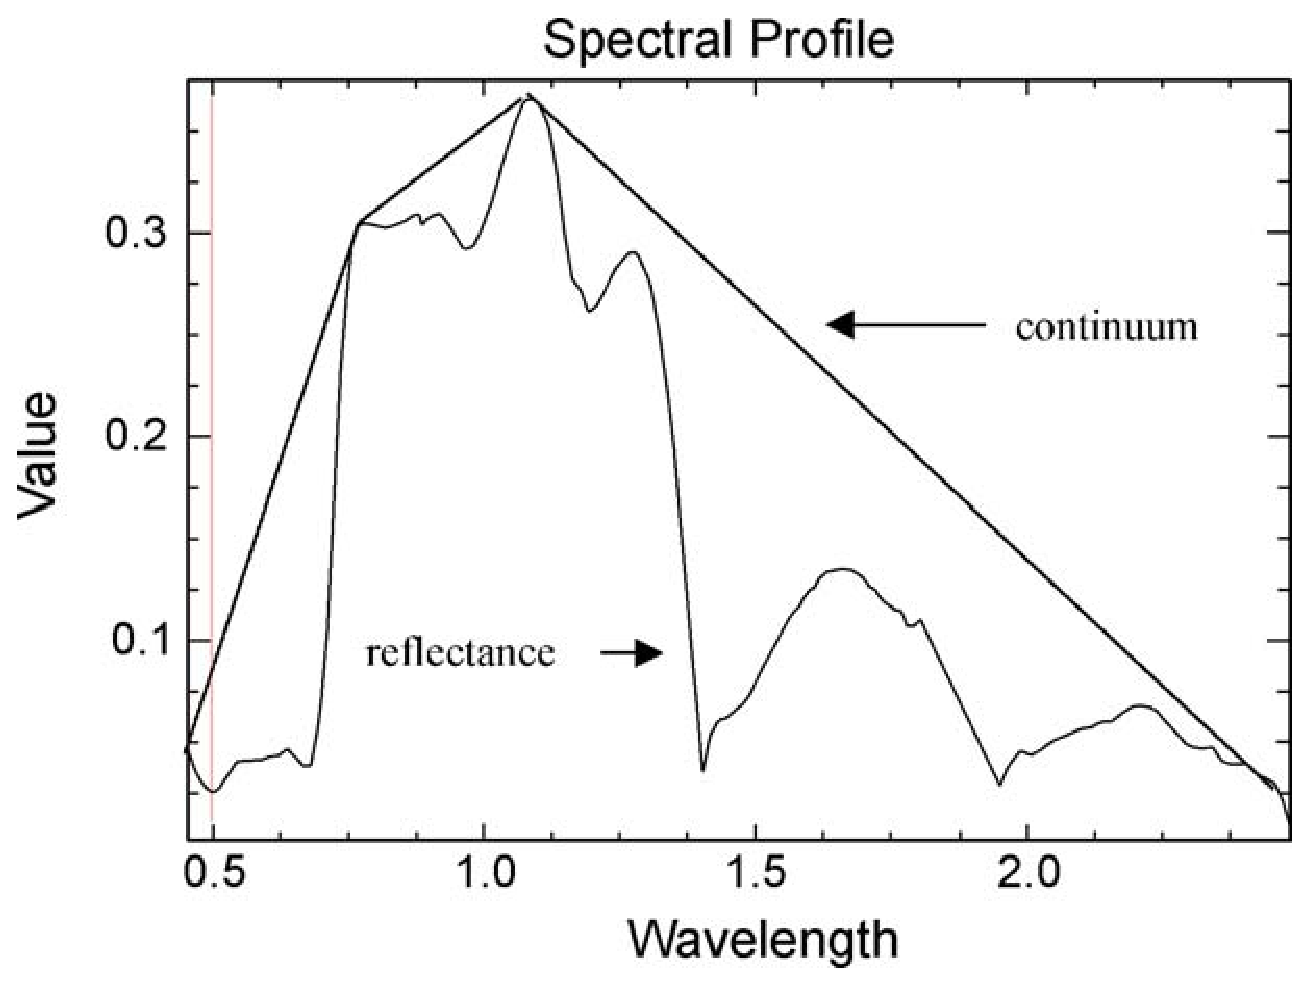
\includegraphics[width=0.9\linewidth]{./Imagenes/CR1.eps}}\\
		\only<3>{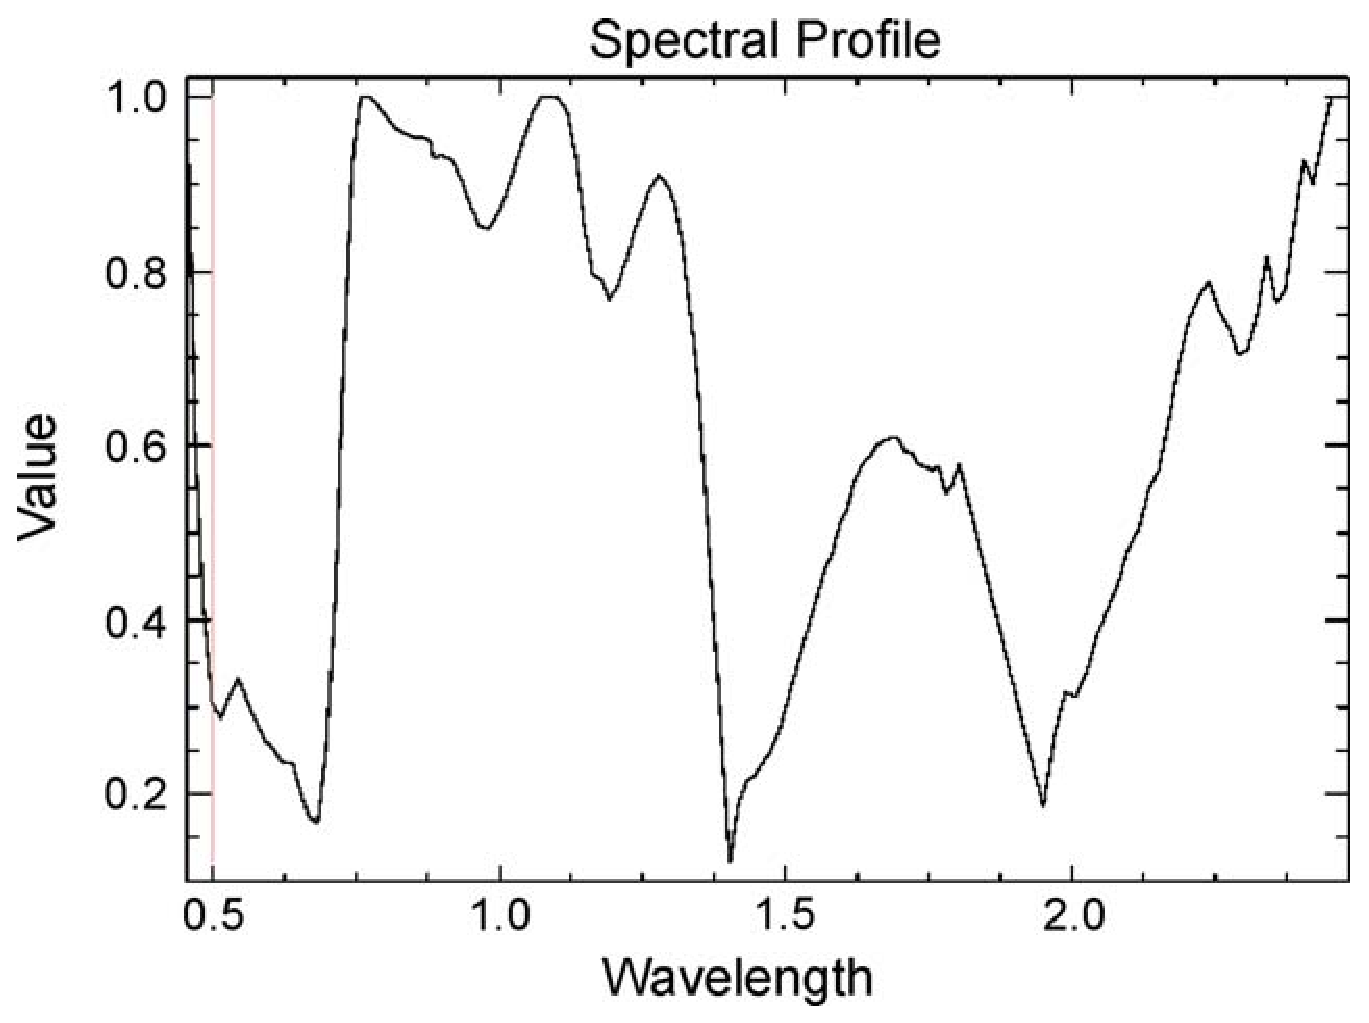
\includegraphics[width=0.9\linewidth]{./Imagenes/CR2.eps}}
		\end{column}
	\end{columns}
\end{frame}

\subsection{Imágenes Landsat}
\begin{frame}
	\begin{block}{}
		contenidos...
	\end{block}
\end{frame}

\section{Conclusiones}
\begin{frame}{Conclusiones}
	contenidos...
\end{frame}

\section{Bibliografía}
\begin{frame}[allowframebreaks]
	\frametitle{Bibliografía}
	
	Para ampliar conocimientos: \nocite{chuvieco2002teledeteccion,schowengerdt2006}
	\bibliographystyle{plain}
	\bibliography{../bibliografia}
\end{frame}

\end{document}